\documentclass[11pt]{article}
\usepackage[a4paper,margin=1in]{geometry}
\usepackage{amsmath,amssymb,amsthm,mathtools}
\usepackage{booktabs}
\usepackage{enumitem}
\usepackage{float}
\usepackage{graphicx}
\usepackage{hyperref}
\usepackage[nameinlink,capitalise]{cleveref}
\usepackage[numbers,sort&compress]{natbib}

\newtheorem{theorem}{Theorem}[section]
\newtheorem{proposition}[theorem]{Proposition}
\newtheorem{corollary}[theorem]{Corollary}
\newtheorem{remark}[theorem]{Remark}
\newcommand{\norm}[1]{\left\lVert#1\right\rVert}
\newcommand{\HS}{\mathfrak S_2}

\title{Nested Arnoldi Residual Closure for Directional Stein Tails\\
\large Repairing the One-Step Propagation Failure}
\author{Liang Wang}
\date{July 2026}

\begin{document}
\maketitle

\begin{abstract}
RH-62 introduced an Arnoldi residual certificate for a directional Stein
tail.  Its projected component was sharp, but the remaining Arnoldi defect
was propagated with an ordinary operator norm; on the RH-60 two-block model
that one-step certificate was worse than the original norm envelope.

RH-63 expands the defect again.  We prove a coherent nested identity in which
all projected residual vectors are added before taking a norm, and only the
terminal unexpanded remainder receives a positive norm bound.  The resulting
certificate is always an upper and is exact when the residual chain reaches
Arnoldi breakdown.  This is a finite-dimensional theorem, independent of
normality.

At horizon $L=32$, the RH-60 two-block model improves from a one-level gain
of $66.41$ to exactly $1$ under a two-level schedule.  A four-step
nonnormal chain improves from $84.05$ to $52.30$, $53.48$, and finally $1$
at four nested levels.  The RH-61 slow/fast surrogate is already nearly
exact at one level, and recursive triangle splitting can make it slightly
more conservative.  The route remains viable, but uniform residual depth,
terminal propagation, and block cross-column fusion are open.  No
physical-family, self-adjoint, arithmetic, or Hilbert--Polya conclusion is
claimed.
\end{abstract}

\noindent\textbf{Keywords:} nested Arnoldi; Krylov residual; Stein tail;
nonnormal operator; directional Hardy energy.

\medskip
\noindent\textbf{MSC 2020:} 47A10; 47B65; 65F35; 93B07; 93D05.

\section{Introduction}

RH-61 identified a sharp difference between the actual directional tail and
the largest-norm Stein envelope.  RH-62 used the source Krylov space to
capture part of that difference, but its residual term still used a
worst-case norm.  The two-block model made the limitation explicit:
one Arnoldi vector gave a gain of about $66$ although the full two-dimensional
Krylov space was exact.

The defect is itself a vector with a structured orbit.  Applying Arnoldi to
that defect and retaining its projected orbit is the smallest coherent
extension.  The construction is related to standard nested Krylov ideas
\citep{Saad2003,GolubVanLoan2013}, but the purpose here is a positive tail
certificate rather than a linear-system solve.

\subsection*{Contributions and boundary}

\begin{enumerate}[leftmargin=2.2em]
 \item We prove the coherent nested Arnoldi identity.
 \item We derive a positive terminal remainder bound.
 \item We prove exactness when the residual chain terminates.
 \item We audit slow/fast, two-block, and nonnormal-chain models and record
       the remaining depth and block-fusion barriers.
\end{enumerate}

All model values are deterministic binary64 calculations.  The
RH-61-calibrated model matches a contraction gap only; it is not a stored
folded-Gaussian production matrix.

\section{Nested residual identity}
\label{sec:identity}

Let $A$ be a square matrix and $z\ne0$.  At level $0$, an Arnoldi relation is
\begin{equation}
 AV_0=V_0H_0+g_0e_{k_0}^*,
 \qquad z=V_0\beta_0.
\label{eq:level-zero}
\end{equation}
Apply the same construction to $g_0$, obtaining
\begin{equation}
 AV_1=V_1H_1+g_1e_{k_1}^*,
 \qquad g_0=V_1\beta_1,
\label{eq:level-one}
\end{equation}
and continue for a finite schedule.  A level with $g_\ell=0$ is a
breakdown and terminates the chain.

\begin{theorem}[Coherent nested identity]
\label{thm:nested}
For every horizon $L\ge0$, recursively substituting the level relations
gives
\begin{equation}
 A^Lz
 = \mathcal A_L+
 \mathcal R_L,
\label{eq:nested-split}
\end{equation}
where $\mathcal A_L$ is the sum of every projected Arnoldi power generated
at every level, with its exact complex coefficient, and $\mathcal R_L$ is a
sum only of terminal unexpanded residual powers.
\end{theorem}

\begin{proof}
At one level, the identity is
\[
 A^Lz=V_0H_0^L\beta_0+
 \sum_{j=0}^{L-1}A^{L-1-j}g_0
 e_{k_0}^*H_0^j\beta_0.
\]
Replace each power of $g_0$ by its level-one identity.  The projected
level-one terms are added to the first term before taking a norm.  Repeating
the substitution at each finite level leaves only terms at the last
unexpanded level.  This is precisely \eqref{eq:nested-split}.
\end{proof}

\begin{proposition}[Positive nested certificate]
\label{prop:positive}
Let $\rho\ge\norm A$.  If the terminal residual terms at level $\ell$ have
coefficients $c_{\ell,j}$ and terminal sources $g_\ell$, then
\begin{equation}
 \norm{A^Lz}
 \le \norm{\mathcal A_L}
 +\sum_{\ell,j}|c_{\ell,j}|\,
 \rho^{u_{\ell,j}}\norm{g_\ell}.
\label{eq:nested-upper}
\end{equation}
Here $u_{\ell,j}$ is the remaining power of the terminal residual.  If the
last residual vanishes, the second term is zero.
\end{proposition}

\begin{proof}
Use the exact coherent decomposition from \cref{thm:nested}, take one norm
of the sum of all projected terms, and use
$\norm{A^u g_\ell}\le\rho^u\norm{g_\ell}$ only on the terminal terms.
\end{proof}

\begin{corollary}[Stein-tail form]
\label{cor:stein}
For $t_L=\sqrt{\kappa}\norm{S^Lz}_{\HS}$, apply
\cref{prop:positive} columnwise and multiply by $\sqrt{\kappa}$.  If every
column terminates, the certificate is exact.
\end{corollary}

\begin{remark}[Remaining wall]
Nested substitution can increase the number of projected terms and still
leaves $\rho^u$ at the terminal level.  Thus depth cannot be declared
uniform without a residual-rank or residual-decay theorem.  The construction
is a route component, not Stage A1 closure.
\end{remark}

\section{Finite-model audit}
\label{sec:audit}

The pilot uses the same three models as RH-62.  A schedule $(1,1)$ means
one Arnoldi vector at the source level and one at the residual level.  The
schedule $(1,1,1,1)$ follows the four-step residual chain.

\begin{table}[H]
\centering
\caption{Nested upper gains at horizon $L=32$.}
\label{tab:gains}
\begin{tabular}{lrrrr}
\toprule
model & one level & two levels & full nested & full primary\\
\midrule
RH-61 slow/fast surrogate & 1.000000 & 1.012274 & 1.000000 & 1.000000\\
RH-60 two-block model     & 66.409450& 1.000000 & 1.000000 & 1.000000\\
four-step nonnormal chain & 84.053899& 52.298902& 1.000000 & 1.000000\\
\bottomrule
\end{tabular}
\end{table}

The two-block row is the decisive repair: its first residual is an
eigenvector, so the second level terminates and the projected terms
reconstruct the exact vector coherently.  The four-step row needs the full
chain for exactness, while intermediate levels still reduce the error.

The slow/fast row illustrates a different issue.  Its one-level certificate
was already nearly exact because the initial vector has a very small slow
component.  A further triangle split can lose a small amount of coherence.
Consequently, nesting is not monotonically better for every source; a
stopping rule must compare the certified upper at each level.

\begin{figure}[H]
\centering
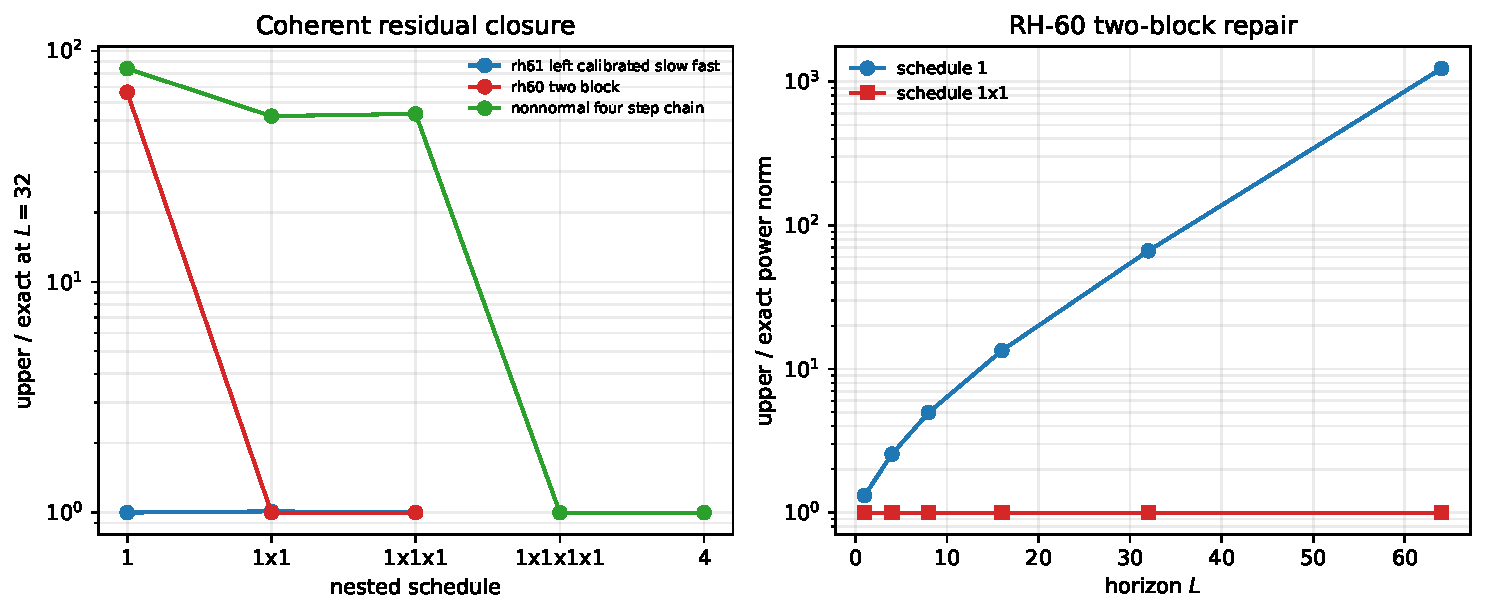
\includegraphics[width=0.98\textwidth]{figures/nested_krylov_closure.pdf}
\caption{Nested residual audit.  Left: the gain at $L=32$ for successive
residual schedules.  Right: the two-block failure of one-level propagation
and its exact repair by one nested level.}
\label{fig:audit}
\end{figure}

A 256-bit Arb calculation verifies the coherent two-level expansion for the
RH-60 two-block model.  The production physical operator is not interval
validated.

\section{Route consequence}
\label{sec:consequence}

RH-63 changes the route boundary identified in RH-62.  The two-block
counterexample is no longer a counterexample to residual recursion:
\begin{equation}
\text{source Krylov}
\longrightarrow
\text{residual Krylov}
\longrightarrow
\text{coherent projected sum}
\longrightarrow
\text{terminal positive tail}.
\label{eq:route}
\end{equation}
Three obligations remain before this can be transferred to the physical
family:

\begin{enumerate}[leftmargin=2.2em]
 \item bound the number of nontrivial residual levels uniformly or
       polylogarithmically;
 \item replace the terminal ordinary norm by a weighted or directional
       residual certificate;
 \item retain cross-column Gram information in a block version.
\end{enumerate}

The next paper should address the second item on the smallest repaired
model.  If a weighted terminal certificate fails there, that failure will be
a sharper obstruction than the original one-step norm gap.

\section{No arithmetic or Hilbert--Polya conclusion}

This paper constructs no self-adjoint operator, no $T\log T$ counting law,
no von Mangoldt or prime-power trace formula, and no completed-zeta
spectral identity.  It makes no Hilbert--Polya or Riemann-hypothesis claim.
The TPC branch is not used.

\section{Reproducibility}

The directory contains the recursive algebra, tests, model pilot, Arb audit,
figures, hashes, and publication artifacts.  The main commands are:
\begin{verbatim}
pytest -q -p no:cacheprovider
python experiments/run_nested_krylov_pilot.py
python experiments/run_arb_nested_audit.py
MPLBACKEND=Agg python experiments/make_figures.py
latexmk -pdf -interaction=nonstopmode -halt-on-error main.tex
\end{verbatim}

The nested identity and positive terminal bound are analytic finite-matrix
results.  The tables are binary64 model evidence.  Stage A1, Stage A4,
uniform residual depth, block cross-column fusion, a self-adjoint
Hilbert--Polya operator, a prime-power trace formula, and a zeta-zero
identity remain open.

\bibliographystyle{plainnat}
\bibliography{references}
\end{document}
